\documentclass[a4paper,twoside,twocolumn]{article}

\usepackage{hyperref}           % For hyperlinks
\usepackage{amsmath, amssymb}     % Use for end of article bullets and eikibooks article
\usepackage[ansinew]{inputenc}    % For "�"
\usepackage{marvosym}             % For currency symbols
\usepackage{eurosym}              % For currency symbols
\usepackage{cwpuzzle}             % For the crossword
\usepackage{rotating}             % For the inverted crossword answers
\usepackage{textcomp}             % For currency symbols
%\usepackage{mathdesign}          % Tried this, it has more currency symbols, but completely changed the default font
\usepackage{cyrillic}             % For the cyrillic letter used for the Serbian dinar
\usepackage{booktabs}             % For tables with TOPRULE, MIDRULE and BOTTOMRULE
\usepackage{graphicx}             % For various illustrations
\usepackage{wrapfig}

% -----------------------------------------------------------------------------------
% Baskerville Definitions

% UK-TUG logo with dropped U
% \def \ukt {UK-T\kern -0,07 em\lower 0,7 ex\hbox{U}\kern 0,07 em G} % Original as 9.1
\def \ukt {UK-T\kern -0,20 em\lower 0,5 ex\hbox{U}\kern -0,08 em G}

\newcommand{\BK}{\textit{Baskerville}}
\newcommand{\ISSUEDATE}{May 2009}

% Used for author name at top of article
\newcommand{\AUTHOR}[1]
{
\textsf{#1} \vspace{1em}
}

\hyphenation{Bas-ker-ville Wiki-pedia Wiki-book Wiki-books}

% -----------------------------------------------------------------------------------
% Definitions for the Constitution
% \newcounter{refa}
% \newcounter{refb}
% \font\manual=manfnt
% \newcommand{\MF}{{\manual META}\-{\manual FONT}}
% -----------------------------------------------------------------------------------

% Applicable for A5
% \voffset    -2cm
% \textheight 16cm

% -----------------------------------------------------------------------------------
% Heading for pages after the first page.
\usepackage{fancyhdr}
\pagestyle{fancy}

% One heading per page, to the margin
\fancyhead[RE]{}
\fancyhead[LE]{\textit{Baskerville}}          % Recto / Odd
\fancyhead[RO]{\textit{Volume 10, Number 1}}  % Verso / Even
\fancyhead[LO]{}

% \lhead{\textit{Baskerville}}
% \rhead{\textit{Volume 10, Number 1}}

\cfoot{-\thepage-}
% -----------------------------------------------------------------------------------

% ============================================================================================
\begin{document}

% -----------------------------------------------------------------------------------
% Define a title page.
\begin{titlepage}
\begin{center}

\vspace{2cm}


\includegraphics[width=0.95\textwidth]{lion.png} \\ [2cm]

\textsc{\large The Annals of the UK-\TeX\ Users' Group} \\[0.2cm]
\href{http://uk.tug.org/}{http://uk.tug.org/} \\[0.2cm]
{\large ISSN 1354-5930}

\vfill

% Bottom of the page
\begin{tabular*}{0.9\textwidth}{@{\extracolsep{\fill}} l c r }
           & Edited by                 &             \\
Vol. 10.1  & Jonathan \textsc{Webley}  & \ISSUEDATE  \\
\end{tabular*}
\end{center}
\end{titlepage}

% -----------------------------------------------------------------------------------
% \setcounter{tocdepth}{1}  % Sections only. 2 turns on sub-sections which throws a new page.
\tableofcontents

% ----------------------------------------------------------------------------------------
\vspace{0.5cm}
\noindent \textbf{\ukt\ Committee 2009}

\begin{itemize}
   % \setlength{\parskip}{0pt} % Scrunch up to fit on A5 page
   \item Jonathan Fine (Chair)
   \item David Crossland (Secretary)
   \item David Saunders (Treasurer)
   \item Joseph Wright (Membership Secretary and Webmaster, co-opted)
   \item John Trapp (Training Officer)
   \item Jonathan Underwood
   \item Charles Goldie
   \item Simon Dales (co-opted)
   \item Jonathan Webley (Baskerville Editor, co-opted)
\end{itemize}
The  committee can be contacted at:
\begin{center}
\href{mailto:uktug-committee@uk.tug.org}{uktug-committee@uk.tug.org}
\end{center}

% ----------------------------------------------------------------------------------------
\section{Editorial}
Welcome to the revived \BK. \BK\ was for many years the journal of \ukt\ and archived copies are available through our website. The \ukt\ committee have decided to start anew publication of \BK\ and I have been co-opted onto the committee as editor. This is the first new issue. Since the purpose of \TeX\ is to produce ``marks on paper'' \BK\ has been printed and posted out; though the PDF version has been emailed out and is also available on the web.

The journal is named after a serif typeface designed in 1757 by John Baskerville. Previous issues of \BK\ used the Baskerville font but this issue uses the default \textit{Computer Modern} font.

This particular issue is somewhat light in content. The quality of future issues will depend on \textit{you}, the membership of \ukt. I do not intent to create all the content myself, and welcome contributions on matters relevant to \TeX\ or \ukt.

I think that a newsletter is central to the well-being of a user group such as ours, and I look forwards to hearing your comments on this issue.

\hfill Jonathan Webley

% ----------------------------------------------------------------------------------------
\section{Events}

\subsection{Bacho\TeX\ 2009}

\begin{wrapfigure}{L}{0.17\textwidth}
    \vspace{-10pt}
    
\includegraphics[width=0.15\textwidth]{bachotex.png}
    \vspace{-10pt}
\end{wrapfigure}

Bacho\TeX\ 2009 is the XVII\textsuperscript{th} Polish \TeX\ Users Group Conference which took place at the traditional \TeX ies' and GUST meeting place, Bachotek near Brodnica, in the north-east of Poland, from 29 April until 3 May 2009 inclusive.

The conference aimed to get a glimpse of the future, and the title was:
\begin{center} ``\textit{\TeX: at a turning point, or at the crossroads?}'' \end{center}

Bogus\l{}aw Jackowski is chairman of the Program Committee which can be contacted at:
\begin{center}
\href{mailto:papers-2009@gust.org.pl}{papers-2009@gust.org.pl}
\end{center}

The conference website is:
\begin{center}
\href{http://www.gust.org.pl/bachotex/2009/main-en.html?set_language=en}{www.gust.org.pl/BachoTeX/2009}   $\blacksquare$
\end{center}

% ----------------------------------------------------------------------------------------
\subsection{Call for \TeX\ Pearls}
GUST, the organisers of Bacho\TeX\, are seeking to continue the tradition of ``The Pearls of \TeX\ Programming''.
Briefly, Pearls are
\begin{itemize}
\item short \TeX, \texttt{MetaFont} or \texttt{MetaPost} macros
\item contain code that is easy to explain and preferably not obvious
\item obscure oddities, exhibiting weird \TeX\ behaviour -- dirty and risky tricks and traps are also welcome
\item not necessarily useful or serious
\end{itemize}

Pearls are collected throughout the year by Pawe\l\ Jackowski, contact:
\begin{center}
\href{mailto:pearls@gust.org.pl}{pearls@gust.org.pl}
\end{center}

Further details can be found at:
\begin{center}
\url{http://www.gust.org.pl/projects/pearls/}  $\blacksquare$
\end{center}

% ----------------------------------------------------------------------------------------
\subsection{Mathematics and Fiction}

\begin{wrapfigure}{L}{0.2\textwidth}
    \vspace{-10pt}
    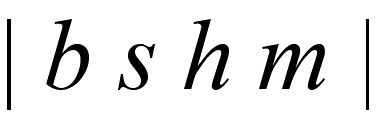
\includegraphics[width=0.17\textwidth]{bshm.jpg}
    \vspace{-10pt}
\end{wrapfigure}

The British Society for the History of Mathematics is hosting a workshop on the relationship between mathematics and fiction on 30-31 May 2009 at Rewley House, Oxford. The workshop will include readings and interviews with writers, talks about the uses of mathematics in fiction, and opportunities for discussion and debate.

One of the contributors is Donald Knuth, the creator of \TeX. He is Professor Emeritus of the Art of Computer Programming at Stanford University and author of the seminal multi-volume work ``The Art of Computer Programming''. Knuth will be talking about his novel ``Surreal Numbers'', published in 1974 and still available on Amazon.

The workshop is organised by
\begin{itemize}
	\item Tony Mann (\href{mailto:A.Mann@gre.ac.uk}{A.Mann@gre.ac.uk})
	\item Noel-Ann Bradshaw (\href{mailto:N.Bradshaw@gre.ac.uk}{N.Bradshaw@gre.ac.uk})
	\item Raymond Flood \\ (\href{mailto:Raymond.Flood@conted.ox.ac.uk}{Raymond.Flood@conted.ox.ac.uk})
\end{itemize}
Further details of the workshop can be found at:
\begin{center}
\url{http://www.bshm.org/meetings/Fiction.html}
\end{center}  $\blacksquare$

% ----------------------------------------------------------------------------------------
\subsection{Euro\TeX\ 2009}

\begin{wrapfigure}{R}{0.12\textwidth}
    \vspace{-10pt}
    
\includegraphics[width=0.09\textwidth]{ntglogo_bw.png}
    \vspace{-10pt}
\end{wrapfigure}

Euro\TeX\ 2009 takes place this year in the Hague, the Netherlands, on 31 August through 4 September 2009, and the conference will focus on educational uses of \TeX, such as manuals, presentations and teaching materials. The conference will be in English.

The fee for \ukt\ members is \euro350, which includes everything except the excursion day (which costs \euro75). In particular it includes accommodation and meals.

The official website is:
\begin{center}
 \href{http://www.ntg.nl/EuroTeX2009/index.html}{www.ntg.nl/EuroTeX2009} $\blacksquare$
\end{center}

% ----------------------------------------------------------------------------------------
\subsection{TUG 2009}
\begin{wrapfigure}{R}{0.12\textwidth}
    \vspace{-20pt} % Remove space at top of logo
    
\includegraphics[width=0.09\textwidth]{tug_bw.jpg}
    \vspace{-10pt} % Remove space at bootom of logo
\end{wrapfigure}

TUG 2009 will take place in Notre Dame, Indiana, from 28-31 July. For the registration form, maps, the proposals already accepted, and more see:
\begin{center}
\href{http://tug.org/tug2009}{http://tug.org/tug2009}
\end{center}

April has several deadlines related to the conference:

\begin{itemize}
	\item 13 April 2009: This is the deadline for abstract submissions; the call for papers is at: 
  \begin{center}
  \href{http://tug.org/tug2009/cfp.html}{http://tug.org/tug2009/cfp.html}
  \end{center}
  Although proposals may be accepted after the deadline, of course potential attendees would like to know what they'll be seeing. So if you'd like to give a talk, please try to submit an abstract by the 13\textsuperscript{th}.
  
  \item 17 April 2009: This is the deadline for bursary applications; for information and the application form see
  \begin{center}
  \href{http://tug.org/bursary}{http://tug.org/bursary} 
  \end{center}
  No late applications will be accepted.
  
  \item 27 April 2009: This is the deadline for the early bird registration discount. After this date, the registration fee will be increased. Register for the conference through Notre Dame's website via this link 
\begin{center}
\url{http://tug.org/tug2009/register.html} $\blacksquare$
\end{center}
\end{itemize}

% ----------------------------------------------------------------------------------------
\subsection{UKUUG Summer Conference 2009}

\begin{wrapfigure}{R}{0.15\textwidth}
    \vspace{-10pt}
    
\includegraphics[width=0.13\textwidth]{ukuug-2006.png}
    \vspace{-10pt}
\end{wrapfigure}

UKUUG is the UK's Unix and Open Systems User Group. Their summer conference will be from Friday 7 August to Sunday 9 August 2009, at the Birmingham Conservatoire (School of Music) near the city centre. For further details see: 
\begin{center}
\href{http://ukuug.org/events/summer2009/}{http://ukuug.org/events/summer2009/} 
\end{center}
One of the streams is a half day session on \textit{\TeX\ and typesetting}.  $\blacksquare$

% ----------------------------------------------------------------------------------------
% \newpage
\section{The Hound}
This is a somewhat easy, cryptic crossword and the solution can be found later in this issue.

\vspace{1em}

\begin{Puzzle}{9}{9}
|[1]C |A |[2]S |E |* |[3]A |[4]W |L |[5]S |.
|U |* |P |* |* |* |O |* |E |.
|[6]S |U |E |* |[7]S |W |E |D |E |.
|P |* |C |* |H |* |B |* |D |.
|* |[8]S |T |E |A |M |E |R |* |.
|[9]B |* |A |* |D |* |G |* |[10]H |.
|[11]U |N |C |L |E |* |[12]O |R |E |.
|G |* |L |* |* |* |N |* |R |.
|[13]S |L |E |D |* |[14]M |E |M |E |.
\end{Puzzle}

\vspace{1em}

\noindent \textbf{Across} \\[2ex]
\begin{tabular}{r l}
 \textbf{1} & In Africa, see a container. (4)\\
 \textbf{3} & These tools are a product of bad laws. (4)\\
 \textbf{6} & Misuse this girl. (3)\\
 \textbf{7} & These weeds for veg. (5)\\
 \textbf{8} & On this ship, the wicked queen mates. (7)\\
 \textbf{11} & Pawnbroker is unclean, almost. (5)\\
 \textbf{12} & Mineral found in store? (3)\\
 \textbf{13} & Poor deals are without a toboggan. (4)\\
 \textbf{14} & Idea came from me, twice. (4)\\
\end{tabular}

\vspace{2ex}

\noindent \textbf{Down} \\ %[2ex]
\begin{tabular}{r l}
 \textbf{1}  & In the discus, perhaps, achieve one's \\
             & peak. (4) \\
 \textbf{2}  & It's a sight, the centilitres in awful cat's \\
             & pee. (9)\\    
 \textbf{4}  & Beg and owe with one, sadly together we \\
             & looked dismal. (9) \\
 \textbf{5}  & Kent's editor knows the issue. (4)\\
 \textbf{7}  & Hades loses a ghost. (5)\\
 \textbf{9}  & These insects cause errors. (4)\\
 \textbf{10} & Sounds like I hear when present. (4)\\
\end{tabular}

% ----------------------------------------------------------------------------------------
% \section{\LaTeX\ Hints \& Tips}
% \textbf{Currency Symbols} \\

\section{Currency Symbols in \LaTeX}

\AUTHOR{Jonathan Webley}

\subsection{The Dollar and the Pound}
Standard keyboards contain the dollar sign (\$), which, of course, is a special symbol in \TeX, so needs to be prefaced with a backslash or oblique: \textbackslash \$. This symbol works properly in both text mode and math mode.

Keyboards also have a pound sign (�), the use of which requires the package \texttt{inputenc}. Additionally, there is a standard command \textbackslash \texttt{pounds}, which renders as \pounds. This symbol works properly in both text mode and math mode.

Additionally, standard \LaTeX\ contains two commands for these signs:

\textbackslash \texttt{textdollar} which renders as \textdollar, and

\textbackslash \texttt{textsterling} which renders as \textsterling.

\subsection{The Euro}

The European Commission specified a euro logo with exact proportions and colours. Whilst the Commission intended the logo to be a prescribed glyph shape, many font designers created their own variants.

\begin{figure}[h!]
  \caption{\textit{Construction of the euro symbol}}
  \centering
    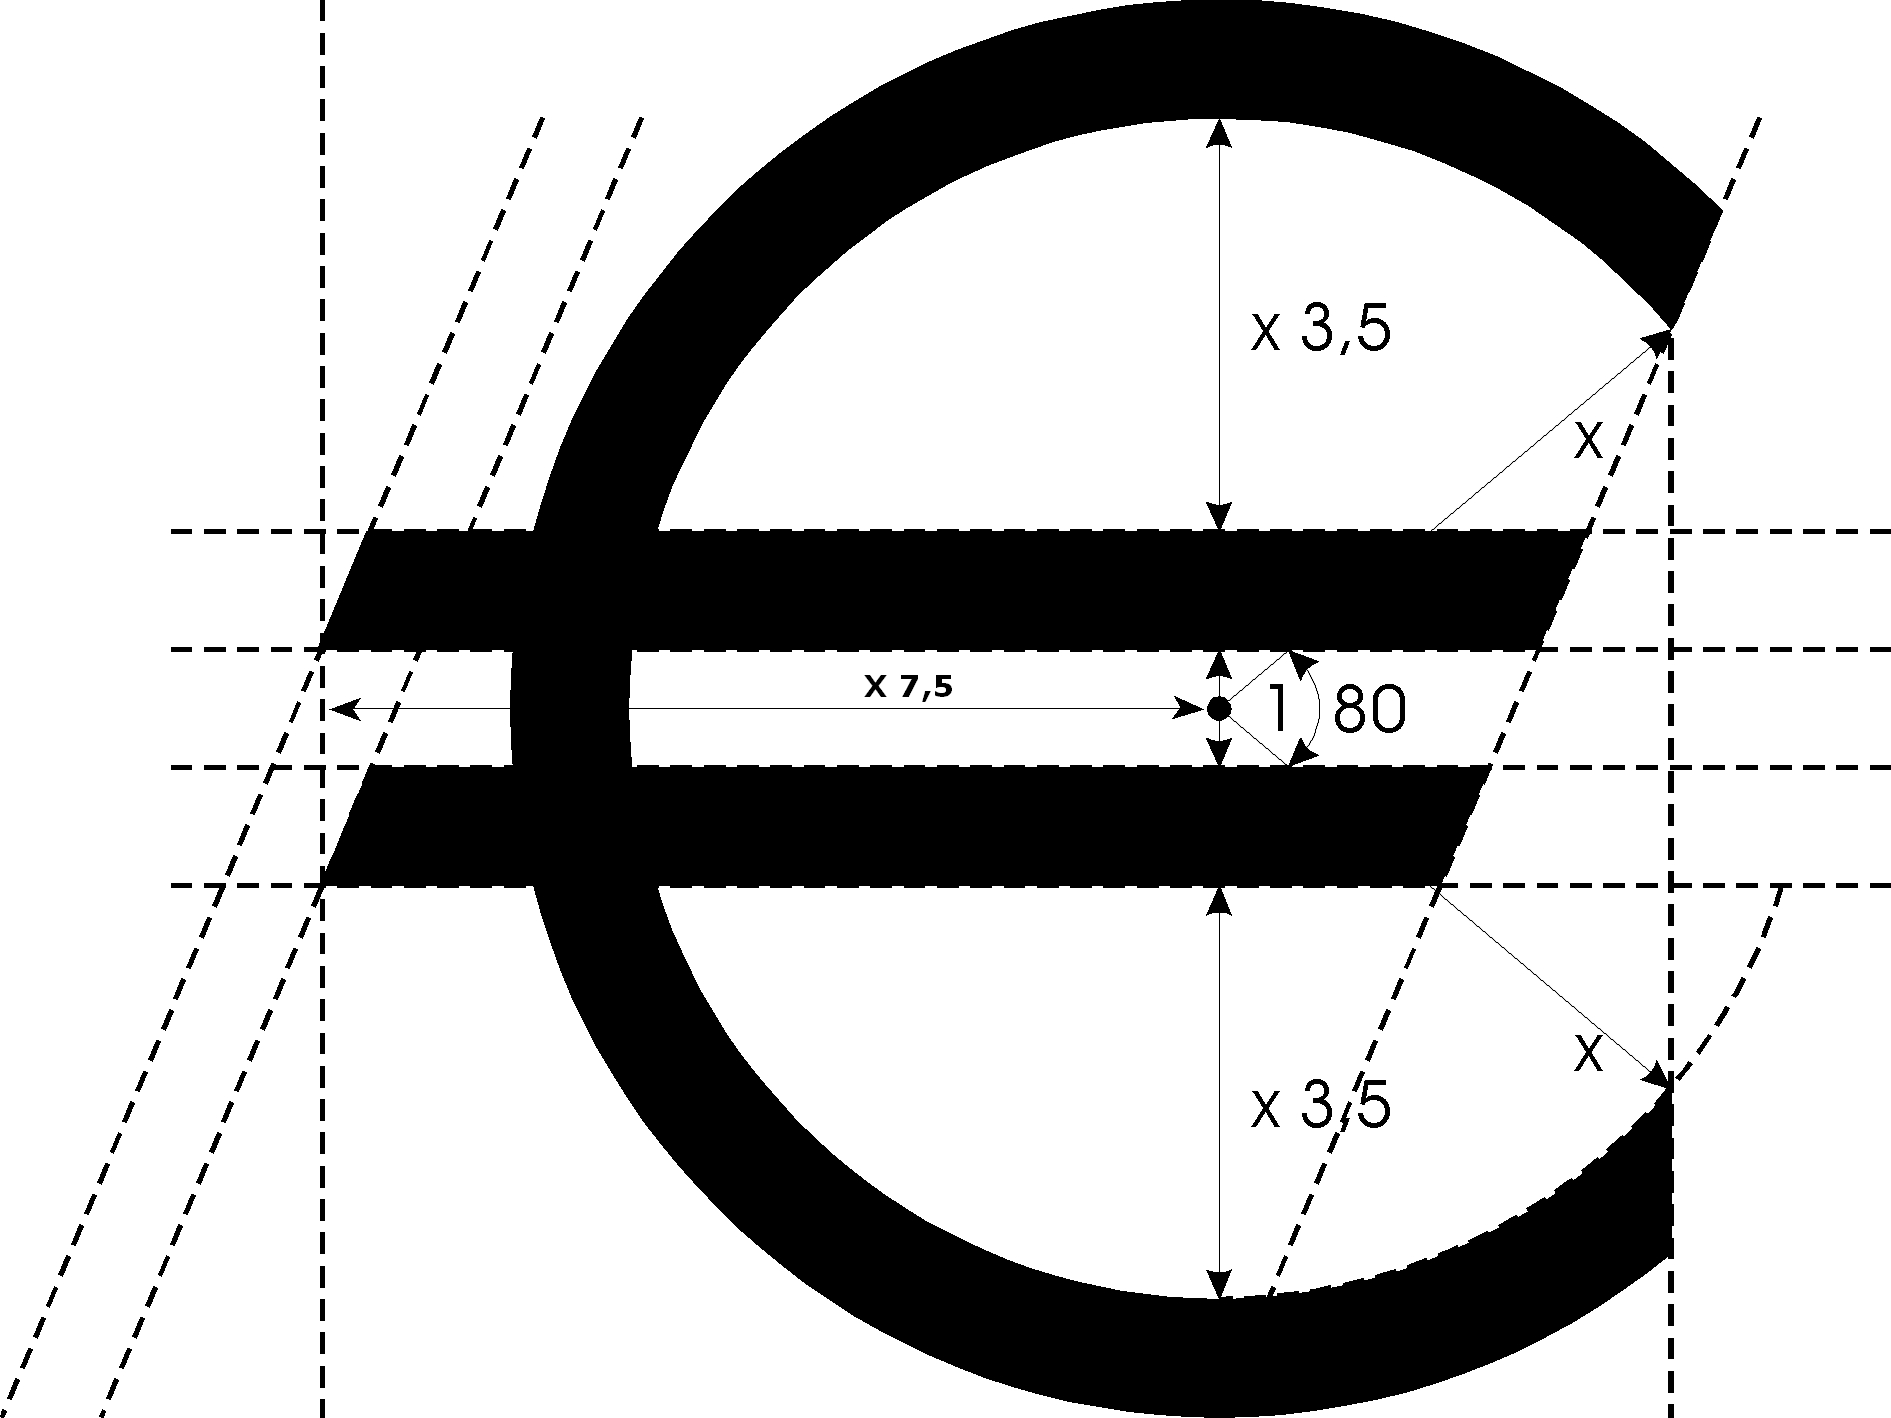
\includegraphics[width=0.45\textwidth]{euro.jpg}
\end{figure}

According to the European Commission:
\begin{quote}
``Inspiration for the \euro\ symbol itself came from the Greek epsilon ($\epsilon$) � a reference to the cradle of European civilisation � and the first letter of the word Europe, crossed by two parallel lines to �certify� the stability of the euro.''
\end{quote}

An approximation to the euro symbol can be created on a typewriter by typing a capital ``C'', backspacing and overstriking it with the equal (``='') sign.

On many computers the euro symbol can be obtained with the \texttt{<ctrl>+<alt>+e} keystrokes.

In \LaTeX\ the euro has its own package, \texttt{eurosym}, which contains these commands:

\medskip

\begin{center}
\begin{tabular}{ l l }
\toprule
\textbf{Symbol} & \textbf{\LaTeX}  \\
\midrule
\geneuro        & \textbackslash \texttt{geneuro} \\
\geneuronarrow  & \textbackslash \texttt{geneuronarrow} \\
\geneurowide    & \textbackslash \texttt{geneurowide} \\
\officialeuro   & \textbackslash \texttt{officialeuro} \\
\bottomrule
\end{tabular}
\end{center}

\medskip

All of these symbols are generated using the ``C'' character of the current body font. The package also contains the command \textbackslash \texttt{euro} which maps to \textbackslash \texttt{officialeuro} but can be altered using a package option.

% --------------------------------------------------------
% Change footnote marker to symbols instead of numbers.
%\renewcommand{\thefootnote}{\fnsymbol{footnote}}
% --------------------------------------------------------

\subsection{And the rest of the World}
The \texttt{textcomp} package includes these symbols: 

\medskip

% I'm not using "xtab" since each currency requires 2 rows and a rule so I found it easier
% just to control the page breaks manually.

\begin{center}
\begin{tabular}{p{2.2cm} p{4.3cm}}
\toprule
\textbf{Symbol} & \textbf{\LaTeX}  \\
\textbf{Name}   & \textbf{Used in} \\
\midrule
\textbaht & \textbackslash \texttt{textbaht} \\
baht & Thailand (THB) \\
\midrule
\textcent & \textbackslash \texttt{textcent} \\
cent & US, Canada \\
\bottomrule
\end{tabular}

\vfill
\newpage

\begin{tabular}{p{2.2cm} p{4.3cm}}
\toprule
\textbf{Symbol} & \textbf{\LaTeX}  \\
\textbf{Name}   & \textbf{Used in} \\
\midrule
\textcentoldstyle & \textbackslash \texttt{textcentoldstyle} \\
cent, old style & \\
\midrule
\textcolonmonetary & \textbackslash \texttt{textcolonmonetary} \\
col\'on  & Costa Rica (CRC), \\
         & El Salvador (SVC), \\
cedi     & Ghana (GHS) \\
\midrule
\textcurrency & \textbackslash \texttt{textcurrency} \\
         & generic currency sign, it is used when no other sign is available. \\
\midrule
\textdollaroldstyle & \textbackslash \texttt{textdollaroldstyle} \\
escudo\footnotemark[1] & formerly Portugal (PTE), \\
                       & Cape Verde (CVE) \\
\midrule
\textdong & \textbackslash \texttt{textdong} \\
dong & Vietnam (VND) \\
\midrule
\texteuro & \textbackslash \texttt{texteuro} \\
euro & Eurozone (EUR) \\
\midrule
\textflorin  & \textbackslash \texttt{textflorin} \\
florin       & Aruba (AWG), \\
or guilder   & Netherlands Antilles (ANG) \\
\midrule
\textguarani & \textbackslash \texttt{textguarani} \\
guarani      & Paraguay (PYG) \\
\midrule
\textlira & \textbackslash \texttt{textlira} \\
lira & Formerly Italy (ITL) and others \\
\midrule
\textnaira & \textbackslash \texttt{textnaira} \\
naira & Nigeria (NGN) \\
\midrule
\textpeso & \textbackslash \texttt{textpeso} \\
peso & Philippines (PHP) \\
\midrule
\textwon & \textbackslash \texttt{textwon} \\
won & South Korea (KRW), \\
    & North Korea (KPW) \\

%\bottomrule
%\end{tabular}
%\vfill
%\begin{tabular}{p{2cm} p{4cm}}
%\toprule
%\textbf{Symbol} & \textbf{\LaTeX}  \\
%\textbf{Name}   & \textbf{Used in} \\

\midrule
\textyen  & \textbackslash \texttt{textyen} \\
yen       & Japan (JPY)  \\
yuan      & China (CNY)  \\
\bottomrule
\end{tabular}
\end{center}

\footnotetext[1]{This version of the dollar sign with two vertical lines is called the cifr�o. Amounts are generally written so that it serves as the decimal separator, such as 20\textdollaroldstyle00 for 20 escudos.}

\medskip

The \texttt{mathdesign} package redefines \textbackslash \texttt{texteuro} to be compatible with these fonts: \textit{Utopia}, \textit{Charter} or \textit{Garamond}.

\medskip

And then there is the \texttt{marvosym} package which has these symbols:

\medskip

\begin{center}
\begin{tabular}{p{2.5cm} p{4cm}}
\toprule
\textbf{Symbol} & \textbf{\LaTeX}  \\
                & \textbf{Use} \\
\midrule
\Denarius   & \textbackslash \texttt{Denarius}\footnotemark[2] \\
            & Obsolete symbol for the German pfennig \\
\EUR        & \textbackslash \texttt{EUR} \\
\EURcr      & \textbackslash \texttt{EURcr} \\
            & Euro compatible with \textit{Courier}. \\
\EURdig     & \textbackslash \texttt{EURdig} \\
            & Euro compatible with \texttt{marvosym} digits. \\
\EURhv      & \textbackslash \texttt{EURhv} \\
            & Euro compatible with \textit{Helvetica}. \\
\EURtm      & \textbackslash \texttt{EURtm} \\
            & Euro compatible with \textit{Times} \textit{Roman}. \\
\EyesDollar & \textbackslash \texttt{EyesDollar} \\
\Shilling   & \textbackslash \texttt{Shilling}\footnotemark[3] \\
\bottomrule
\end{tabular}
\end{center}

In conclusion, \LaTeX\ caters for all common, and some not so common, currency symbols. Unicode, however, has a few additional ones, and is far better documented.  $\blacksquare$

% \vfill

\footnotetext[2]{The denarius was a Roman coin. The dinar is a descendant of the denarius and is used, or was formerly used, by several countries. However, Serbia, for example, use the cyrillic De (\textcyrrm{D}) letter for the dinar.}
\footnotetext[3]{This symbol resembles a beta ($\beta$) but I belive it to be more akin to the German Eszett (\ss). It is possibly a symbol for the schilling, the pre-euro currency of Austria.}

% ----------------------------------------------------------------------------------------
\section{Wikibooks}

\AUTHOR{Jonathan Webley}

\subsection{Wikis}
Wikis are the backbone of Web 2.0 - collaborative websites with dynamic, user-driven content.

The Wikimedia Foundation hosts many wiki projects in many languages using its MediaWiki application. These wikis all have the same, simple ethos - information is free. Notoriously, any anonymous amateur can contribute and there is no guarantee that information is either correct, complete or legal. 

\begin{center}

\includegraphics[width=0.38\textwidth]{Wikipedia.png}
\end{center}

\medskip

But surprisingly the concept works and the flagship project, Wikipedia, is a huge success. There are many editors making small contributions and a few who spend hours and hours editing. Minor errors are easily fixed, articles are continually kept up to date, and an army of volunteers check for vandalism and enforce standards. Copyright issues are dealt with, facts are checked and malicious contributors blocked. Wikipedia has readable and useful articles covering many more topics and in more depth than any paper encyclop\ae dia.

\subsection{\LaTeX\ and MediaWiki}
The MediaWiki software supports \LaTeX. It uses a limited subset of \AmS-\LaTeX\ generating either PNG images or simple HTML mark-up, depending on user preferences and the complexity of the expression.

In MediaWiki, \LaTeX\ is enclosed within the tags \texttt{<math>} and \texttt{</math>}; there is a button to insert these into the edit box. So a simple equation, such as Euler's formula, would be entered as
\begin{center}
\texttt{<math>e\^\{i\textbackslash pi\} + 1 = 0</math>}
\end{center}

And should appear on screen as:
\[
e^{i\pi} + 1 = 0
\]

Maxwell's equations provide an example requiring aligned equations, and are entered as:

\medskip

\noindent \texttt{<math> \\
\textbackslash begin\{align\} \\
\textbackslash nabla \textbackslash cdot \textbackslash mathbf\{D\} \&= \textbackslash rho\_f \textbackslash \textbackslash \\
\textbackslash nabla \textbackslash cdot \textbackslash mathbf\{B\} \&= 0 \textbackslash \textbackslash \\
\textbackslash nabla \textbackslash times \textbackslash mathbf\{E\} \&= \\
        -\textbackslash frac\{\textbackslash partial \textbackslash mathbf\{B\}\} \{\textbackslash partial t\} \textbackslash \textbackslash \\ 
\textbackslash nabla \textbackslash times \textbackslash mathbf\{H\} \&= \textbackslash mathbf\{J\}\_f + \textbackslash frac\{\textbackslash partial \textbackslash mathbf\{D\}\} \{\textbackslash partial t\} \\
\textbackslash end\{align\} \\
</math>}

\medskip

And these appear as:
\begin{align*}
\nabla \cdot \mathbf{D} &= \rho_f \\
\nabla \cdot \mathbf{B} &= 0 \\
\nabla \times \mathbf{E} &= -\frac{\partial \mathbf{B}} {\partial t} \\
\nabla \times \mathbf{H} &= \mathbf{J}_f + \frac{\partial \mathbf{D}} {\partial t}
\end{align*}

Equations are not automatically numbered, and the \texttt{align*} environment is neither available nor required.

\subsection{Wikibooks}
Wikipedia has several sister projects and Wikibooks is one of the more useful of these. Whereas Wikipedia hosts many encyclop\ae dic articles, Wikibooks hosts fewer, longer articles or books, with a more connected narrative and chapters that would normally be read in order. Each Wikibook aims to be a definitive reference work -- though few achieve this.

The Wikipedia article on \LaTeX\ is short and covers only a few subjects such as the history of \LaTeX\ and licensing issues. But in Wikibooks, the \LaTeX\ book has over 30 chapters (or pages) and appendices. Some of these are substantital and considered ``complete'', others are bare stubs. The chapters cover various subjects including tables, graphics, indexing and maths environments. There is a small index and a glossary and contains material both for the beginner and the expert. Wikipedia concentrates on the \textit{why} and Wikibooks on the \textit{how}.

Other sister projects include Wiktionary, a dictionary, which ultimately aims to define all words in all languages. Wikiversity is a ``university'', which aims to have learning resources such as courses and tests, but has only a limited amount of material on \LaTeX.

\subsection{Featured Book}
The Wikibook on \LaTeX\ is a featured book. Out of the thousands of Wikibooks, less than 70 are featured. A random selection of featured books appears on the front page of Wikibooks. Featured books have an exceptionally high quality, lots of content and are well-formatted. \LaTeX\ was nominated in April 2007, garnered seven supporting votes and achieved featured status in May 2007. 

\begin{center}

\includegraphics[width=0.40\textwidth]{Wikibooks-logo-en-bw.png}
\end{center}

The \LaTeX\ book is listed as the 4\textsuperscript{th} most popular Wikibook. Books are ranked by their most popular page, which for \LaTeX\ is the front page -- the contents page. This page averaged over 1000 hits per day over a sample period in 2008. Several other pages (or chapters) from this book also made it into the top 20.

Wikibooks, unlike most of the other wiki projects, has this year introduced reviewed pages. Reviewing assesses pages with regard to readability, accuracy and depth. A reviewed page is considered to be a stable version of that page. Reviewing can only be carried out by ``editors''. Editor status is automatically granted to contributors who have met various criteria such as having made sufficient edits and having a confirmed email address. All pages need to be reviewed, and re-reviewed if changed. In the \LaTeX\ Wikibook many pages still require to be reviewed.

\subsection{Conclusion}
All wiki content must be seen as a work-in-progress. If you don't like it - you can fix it or improve it or start again from scratch. The \LaTeX\ Wikibook has several small chapters which need to be expanded; other chapters need to be enhanced, and more chapters could easily be added. There also two very short and incomplete Wikibooks on \TeX.

In conclusion, the \LaTeX\ Wikibook is a reasonably good online resource, and one that can only get better, especially with our support.

\subsection{Links}
\begin{description}
  \item[\LaTeX\ Wikibook:]                       \hfill \\ \url{http://en.wikibooks.org/wiki/LaTeX}
  \item[\TeX\ Wikibook:]                         \hfill \\ \url{http://en.wikibooks.org/wiki/TeX}
  \item[\TeX\ for the Impatient Wikibook:]       \hfill \\ \url{http://en.wikibooks.org/wiki/TeX_for_the_Impatient}
  \item[Wikibooks guide to reviewing pages:]     \hfill \\ \url{http://en.wikibooks.org/wiki/Using_Wikibooks/Reviewing_Pages}
  \item[Wikpedia article on \LaTeX:]             \hfill \\ \url{http://en.wikipedia.org/wiki/LaTeX}
  \item[Wikipedia help on displaying formul\ae:] \hfill \\ \url{http://en.wikipedia.org/wiki/Help:Displaying_a_formula}
\end{description}
$\blacksquare$

% ----------------------------------------------------------------------------------------
\section{The Hound Answers}
\noindent \textbf{Across} \\
\begin{turn}{180} 
 8. steamer,
11. uncle,
12. ore,
13. sled,
14. meme
\end{turn} \\
\begin{turn}{180}
 1. case,
 3. awls,
 6. Sue,
 7. swede,
\end{turn} \\

\noindent \textbf{Down} \\
\begin{turn}{180}
4. woebegone,
5. seed, 7. shade, 9. bugs, 10. here
\end{turn} \\
\begin{turn}{180}
1. cusp, 2. spectacle, 
\end{turn}

% -----------------------------------------------------------------------------------
\section{Contributions}
\noindent All contributions should be sent to:
\begin{center}
\href{mailto:baskerville@uk.tug.org}{baskerville@uk.tug.org}
\end{center}

Articles on any area of \TeX, its friends, \ukt\ or related topics are very welcome: the Committee is particularly keen to publish articles with a UK \textit{flavour}. Send in your comments on this issue; your suggestions, letters, thoughts, tips and hints, articles, jokes, questions, requests for help, jobs � anything relevant will be considered for publication. Also considered for publication are cartoons and puzzles. $\blacksquare$

% The deadline for the next issue is [\textbf{DATE}]. 

\end{document}
